\documentclass[12pt, a4paper]{article}
\usepackage[utf8]{inputenc}
\usepackage{physics}
\usepackage{graphicx}
\usepackage{amsmath}
\usepackage{cancel}

\usepackage{MnSymbol}%
\usepackage{wasysym}%
%code color
\usepackage{listings}
\usepackage{xcolor}

\begin{document}
	Mr. Phiphat Chomchit 630631028
	\begin{center}
		\textbf{Homework: Search}
	\end{center}
	
	\begin{enumerate}
		\item 3 Jugs\\
		 “You have three jugs, measuring $12$ gallons, $8$ gallons, and $3$ gallons, and a water faucet.  You can fill the jugs up or empty them out onto the ground, or pour from one jug $(A)$ to another $(B)$ until $(1)$ the target jug $(B)$ is full, or $(2)$ the source jug is empty $(A)$. You need to measure out exactly one gallon.”
		
		\begin{itemize}
			\item States: Water level in 3 jugs. Let jugs be $J_{12}, J_{8}, J_{3}$. Variables are $W_{12}, W_{8}, W_{3}$ water level of each jugs s.t.\\   $0 \leq W_{12} \leq 12, 0 \leq W_{8} \leq 8, 0 \leq  W_{3} \leq 3$. \\ State is $W = \{W_12, W_8, W_3\}$
			
			\item Actions:
			\begin{itemize}
				\item $Fill(J_x)$: fill jux x from the faucet.\\ \textbf{Precondition :} $J_x$ is not full.
				
				\item $Empty(J_x)$ empty jux x.\\
				\textbf{Precondition :} $J_x$ is not empty.
				
				\item $Pour(J_x, J_y)$: pour water from jug x to jug y.\\
				\textbf{Precondition :} $J_x$ is not empty and $J_y$ is not full.
			\end{itemize}
		\item Transition Model:
		\begin{itemize}
			\item $Fill(J_x): W_x = x$.
			\item $Empty(J_x): W_x = 0$.
			\item $Pour(J_x, J_y):$\\
			$if (y - W_y > W_x)\{\\
			 W_y = W_x + W_y\\
			W_x = 0\\
			\} else\{\\
			W_y = y\\
			W_x = W_x - (y - W_y)
			\}$
			
		\end{itemize}
	
		\item Goal Test:
		\begin{itemize}
			\item $SUM(W) == 1$
			\item $W_{12} == 1 \quad OR\quad W_{8} == 1 \quad OR\quad W_{3} == 1 $
		\end{itemize}
		\item Step cost:
		\begin{itemize}
			\item $1$ per action.
		\newpage
		\end{itemize}
		\item Path cost:
		\begin{itemize}
			\item Sum of step costs in the path.
		\end{itemize}
		\item Answers (Iterative Deepening Depth First Search):
		\begin{itemize}
			\item Answers 1:\\
			$\{0, 0, 0\} \xrightarrow{Full(J_{12})} \{0, 0, 12\} \xrightarrow{Pour(J_{12}, J_{8})} \{0,8,4\} \xrightarrow{Pour(J_{12}, J_{3})} \{3,8,1\} \xrightarrow{Empty(J_{8})} \{3,0,1\} \xrightarrow{Empty(J_{3})} \{0,0,1\}$\\ 
			
			\item Answers 2:\\
			$\{0, 0, 0\} \xrightarrow{Full(J_{12})} \{0, 0, 12\} \xrightarrow{Pour(J_{12}, J_{3})} \{3,0,9\}
			\xrightarrow{Pour(J_{12}, J_{8})} \{3,8,1\} \xrightarrow{Empty(J_{8})} \{3,0,1\} \xrightarrow{Empty(J_{3})} \{0,0,1\}$\\
			
			\item Answers 3:\\
			$\{0, 0, 0\} \xrightarrow{Full(J_{12})} \{0, 0, 12\} \xrightarrow{Pour(J_{12}, J_{8})} \{0,8,4\}
			\xrightarrow{Empty(J_{8})} \{0,0,4\} \xrightarrow{Pour(J_{12}, J_{3})} \{3,0,1\} \xrightarrow{Empty(J_{3})} \{0,0,1\}$\\
			
			\item Answers 4:\\
			$\{0, 0, 0\} \xrightarrow{Full(J_{12})} \{0, 0, 12\} \xrightarrow{Pour(J_{12}, J_{3})} \{3,0,9\} \xrightarrow{Empty(J_{3})} \{0,0,9\} \xrightarrow{Pour(J_{12}, J_{8})} \{0,8,1\} \xrightarrow{Empty(J_{8})} \{0,0,1\}$\\
		\end{itemize}
		\end{itemize}
	
	\newpage
	\item Cryptarithmetic
	\begin{center}
		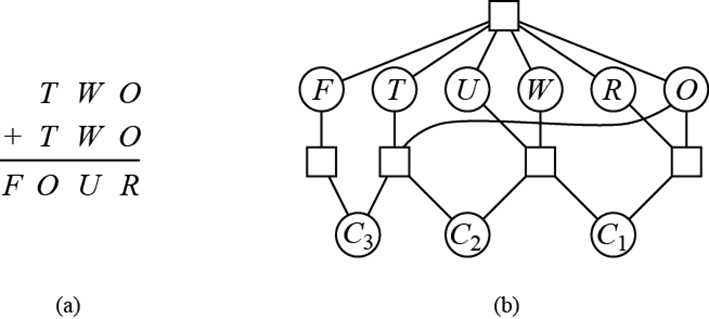
\includegraphics[scale=0.8]{Picture1.png}
	\end{center}
	Problem is shown on $(a)$. Each letter is a digit. No two letters can have the same digit. Hypergraph $(b)$ shows constraints between variables, where $C1, C$2 and $C3$ are carries, and can have value between $0$ and $1$. Find the correct digit for each letter.
	\begin{itemize}
		\item Variables : $F, T, U, W, R, O, C_1, C_2, C_3$
		
		\item Domains:
		\begin{itemize}
			\item $\{0,1,2,3,4,5,6,7,8,9\}$ for $F, T, U, W, R,$ and $O$
			\item ${0, 1}$ for carry variables $C_1, C_2$ and $C_3$
		\end{itemize}
		\item Constranints: $Alldiff (F,T,U,W,R,O)$
		\begin{itemize}
			\item $O + O = R + 10C_1$
			\item $C_1 + W + W = U + 10C_2$
			\item $C_2 + T + T = O + 10 C_3$
			\item $C_3 = F, T \not = 0, F\not = 0$
		\end{itemize}
	 \item Answer:
	 \begin{itemize}
	 	\item[$\blacksquare$] Find singleton domain :\\
	 	From $C_3 = F$ and $F \not = 0$ and $C_3 \in \{0,1\} \Rightarrow F = 1$
	 	
	 	\item[$\blacksquare$] Minimum Remaining Values :\\
	 	From $C_1, C_2 \in \{0,1\}$, We assigned $C_1 = C_2 = 1$, so
	 	\begin{align*}
	 		O + O &= R + 10 \Rightarrow O \geq 5 \\
	 		W + W &= U + 9 \Rightarrow W \geq 5, U \geq 3\\
	 		T + T &= O + 9 \Rightarrow T \geq 5
	 	\end{align*} 
 	
	 	\item[$\blacksquare$] Minimum Remaining Values :\\
	 	From $O, W, T \in \{5,6,7,8,9\}$ and $U \in \{3,4,5, 6, 7, 8, 9\}$ and $R \in \{0, 1, \cdots, 8, 9\}$. We assigned $O = 5$, so $T = 7$ and $R = 0$
	 	
	 	\item[$\blacksquare$] Minimum Remaining Values :\\
	 	From $W \in \{6, 8, 9\}$ and $U \in \{3, 4, 6, 8, 9\}$.
	 	We assigned $W = 6$ so $U = 3$
	 	
	 	\item[$\blacksquare$] Check Answer:
	 	Our answer is 
	 	\begin{align*}
	 		F &= 1\\
	 		T &= 7\\
	 		U &= 3\\
	 		W &= 6\\
	 		R &= 0\\
	 		O &= 5\\
	 		TWO &= 765\\
	 		FOUR &= 1530\\
	 		TWO + TWO &= 765+765 = 1530 = FOUR
	 	\end{align*}
	 \end{itemize}
	\end{itemize}
	\end{enumerate}
\end{document}